\chapter[Single-Crystal EPR on FeFe-Hydrogenase]{Single-Crystal EPR on the H$_{ox}$ stable catalytic intermediate of [FeFe]-Hydrogenase\blfootnote{Portions of this text are from J.~W.~Sidabras, J.~Duan, M.~Winkler, T.~Happe, R.~Hussein, A.~Zouni, D.~Suter, A.~Schnegg, W.~Lubitz, E.~J.~Reijerse, Sci. Adv., 10~(5) (2019), eaay1394. and is reproduced under the CC BY-NC license.}}
\setcitestyle{citesep={,\,\thechapter.}}

Nature has evolved enzymes with various metallic cofactors (metallo-enzymes) to efficiently catalyze energy conversion reactions. These enzymes, which include, for example, photosystem II oxygen-evolving complex\cite{CoxOEC}, hydrogenases\cite{lubitzhyd}, nitrogenases\cite{Hoffman2014rev}, and CO dehydrogenase\cite{C5CS00182J}, employ first-row transition metals to perform their catalytic functions. One of the main challenges is to fully understand these enzymatic mechanisms and provide a basis for cheap, robust, and highly active molecular catalysts designed for practical applications. \cite{Lewis15729} The ultimate goal is to alleviate the requirement of noble metals, such as platinum, that limit the scalability of current technology. This important biophysical and biochemical research seeks metallo-enzyme based and inspired systems as an interesting route to advance towards the future of clean energy and efficient energy storage. \cite{schlogl2012chemical}

The catalytic cycle of redox enzymes often contain paramagnetic intermediates and EPR is the method of choice used to study these occurrences. Through EPR experiments, information on the magnetic and geometrical structure of the active site can be obtained. EPR spectroscopy can probe isolated intermediates in the catalytic cycle when either a single unpaired electron or multiple unpaired electrons with magnetic couplings are present in the ground state. Fundamentally understanding such enzymes is of broad biochemical and biophysical importance as scientists move towards bioengineering mimics of nature’s most elusive chemistry. \cite{WATANABE20171}

One such interesting class of metallo-enzymes are the hydrogenases\cite{lubitzhyd} which catalyze the conversion of molecular hydrogen H$_2$, such that,
\begin{equation}
    \text{H}_2 \rightleftharpoons 2 \text{H}^+ + 2\text{e}^{\text{-}}.
\end{equation}
Hydrogenases are key enzymes in many organisms for hydrogen metabolism regulation in the cell or are used as electron donors for processes further down energy conversion pathways. The hydrogenase enzyme family has three distinct active-sites with different mechanistic hydrogen conversion. These mechanisms utilize either a single-iron center [Fe], a bi-nuclear iron [FeFe], or a nickel-iron [NiFe] active site for catalysis.

For hydrogenases, specifically [NiFe]-hydrogenase, the single-crystal EPR strategy has been very successful. \cite{NiFe1996,NiFe2000,NiFe2003,NiFeRev2007} The active site of this enzyme harbors a [NiFe] binuclear cluster in which the iron carries two cyanide (CN$^-$) and one carbon-monoxide (CO) ligand. The metals are bridged by two cysteine thiols and the nickel center is further coordinated by two cysteine thiolate side groups. The paramagnetic states all originate from the nickel center, while the iron center remains Fe(II) during the catalytic cycle. \cite{lubitzhyd} The open-coordination site between the two metals can be occupied by an oxygen species leading to the inactive oxidized states or a hydride, which is the key intermediate in the catalytic cycle. \cite{NiFeRev2007} For all these species the $g$-tensor magnitude and orientation was determined and analyzed in terms of ligand-field theory and verified using quantum chemical calculations providing fundamental insight into the electronic structure and the dependence on the first ligand-sphere. \cite{Ping2005,Gasteljp0573902,NiFeRev2007,LubitzNiFe2016} The [NiFe]-hydrogenase crystals in these studies were relatively large (2 $\times$ 0.5 $\times$ 0.5~mm$^3$) enabling measurements in standard X-band probeheads with measuring time of 2-3 hours per angle, stepping over 180 degrees. However, even with the large crystal volume, ESEEM and HYSCORE experiments on [NiFe]-hydrogenase were only published in frozen solution with volumes of 50-200~$\mu$L and experimental times upwards of 2 hours for each experiment. \cite{NiFeRev2007} 

\begin{figure}[htpb]
\centering
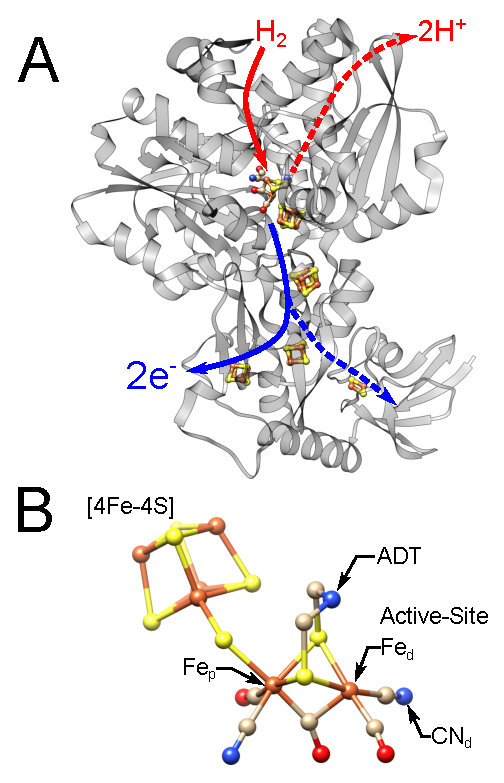
\includegraphics{Kapitel/Ch1-images/CpI-geometry.eps}
\caption[Crystal structure of \textit{Clostridium pasteurianum} (CpI).]{A) Crystal structure of \textit{Clostridium pasteurianum} (CpI) from PDB ID 4XDC. \cite{FeFeCry} The [Fe-Fe]-Hydrogenase CpI is a 64~kDa protein with four [4Fe-4S] clusters and one [2Fe-2S] cluster. The iron-sulfur  clusters  are involved  in  the electron\-/transfer  pathway (solid blue). A [2Fe-2S] cluster is found symmetric to the [4Fe-4S] pathway (dashed blue) and is believed to ``tune'' the redox potentials of the nearby [4Fe-4S] clusters. There exists a proton (2H$^+$;dashed red) and hydrogen (H$_2$; solid red) transfer channel. The active-site, or the H-cluster, resides at the top in this view and is expanded to show the H-cluster structure. B) Within the H-cluster, the proximal iron (Fe$_p$) and distal iron (Fe$_d$) of the [FeFe]-hydrogenase is shown. Fe is orange, S is yellow, N is blue, O is red, and C is beige.}
 \label{fig:CpIGeo}
\end{figure}

Of great interest is the bi-nuclear [FeFe]-hydrogenase. \cite{PETERS20151350} These enzymes have turn-over frequencies over 10,000 s$^{\text{-1}}$\cite{CatalyticTOF} and provide a potential route to sustainable hydrogen production. The proposed crystal structure of one such hydrogenase from \textit{Clostridium pasteurianum} (CpI) highlighting the active site and electron-transfer pathway is shown in Fig.~\ref{fig:CpIGeo}A. \cite{FeFeCry} The electron-transfer pathway involving accessory iron-sulfur clusters is indicated as a solid blue arrow. In CpI, a [2Fe-2S] cluster is found symmetric to the electron-transfer pathway, illustrated as a dashed blue line, and is believed to ``tune'' the redox potentials of the [4Fe-4S] clusters. \cite{PetersPotentials} 

The [FeFe]-hydrogenase active-site, shown in Fig.~\ref{fig:CpIGeo}B, carries a [4Fe-4S] cluster linked via a cysteine ligand connecting the [2Fe]-cofactor molecule. The [2Fe]-cofactor contains an iron atom proximal (Fe$_p$) and one distal (Fe$_d$) to the [4Fe-4S] cluster. Each iron carries a cyanide (CN$^-$) and one carbon-monoxide (CO) ligand. The two irons share a bridging carbon-monoxide ($\mu$CO). Additionally, the two iron atoms are bridged by a 2-aza-propane 1,3-dithiolate (ADT) ligand. The [FeFe]-hydrogenase active site is known as the H-cluster and has a total of six iron atoms at various redox states in the catalytic cycle. In the vicinity of the H-cluster, there exists proton (2H$^+$; illustrated as a dashed red line) and molecular hydrogen (H$_2$; illustrated as a solid red line) channels for gas exchange. Through many spectroscopic techniques, such as Fourier Transform Infra-Red (FTIR), EPR, Nuclear Magnetic Resonance (NMR), M\"o\ss{}bauer, Raman, and Nuclear resonance vibrational (NRVS), a convincing catalytic cycle, shown in Fig.~\ref{fig:FeFeCatCycle}, has been hypothesized. \cite{lubitzhyd,NRVS2017,sommer2017} However, the full $g$-tensor and the hyperfine-tensor, including angular information of the active site are still elusive. More work must be done to fully understand the catalytic mechanism and relate it to quantum chemical calculations. 

\begin{figure*}[htbp]
\centering
 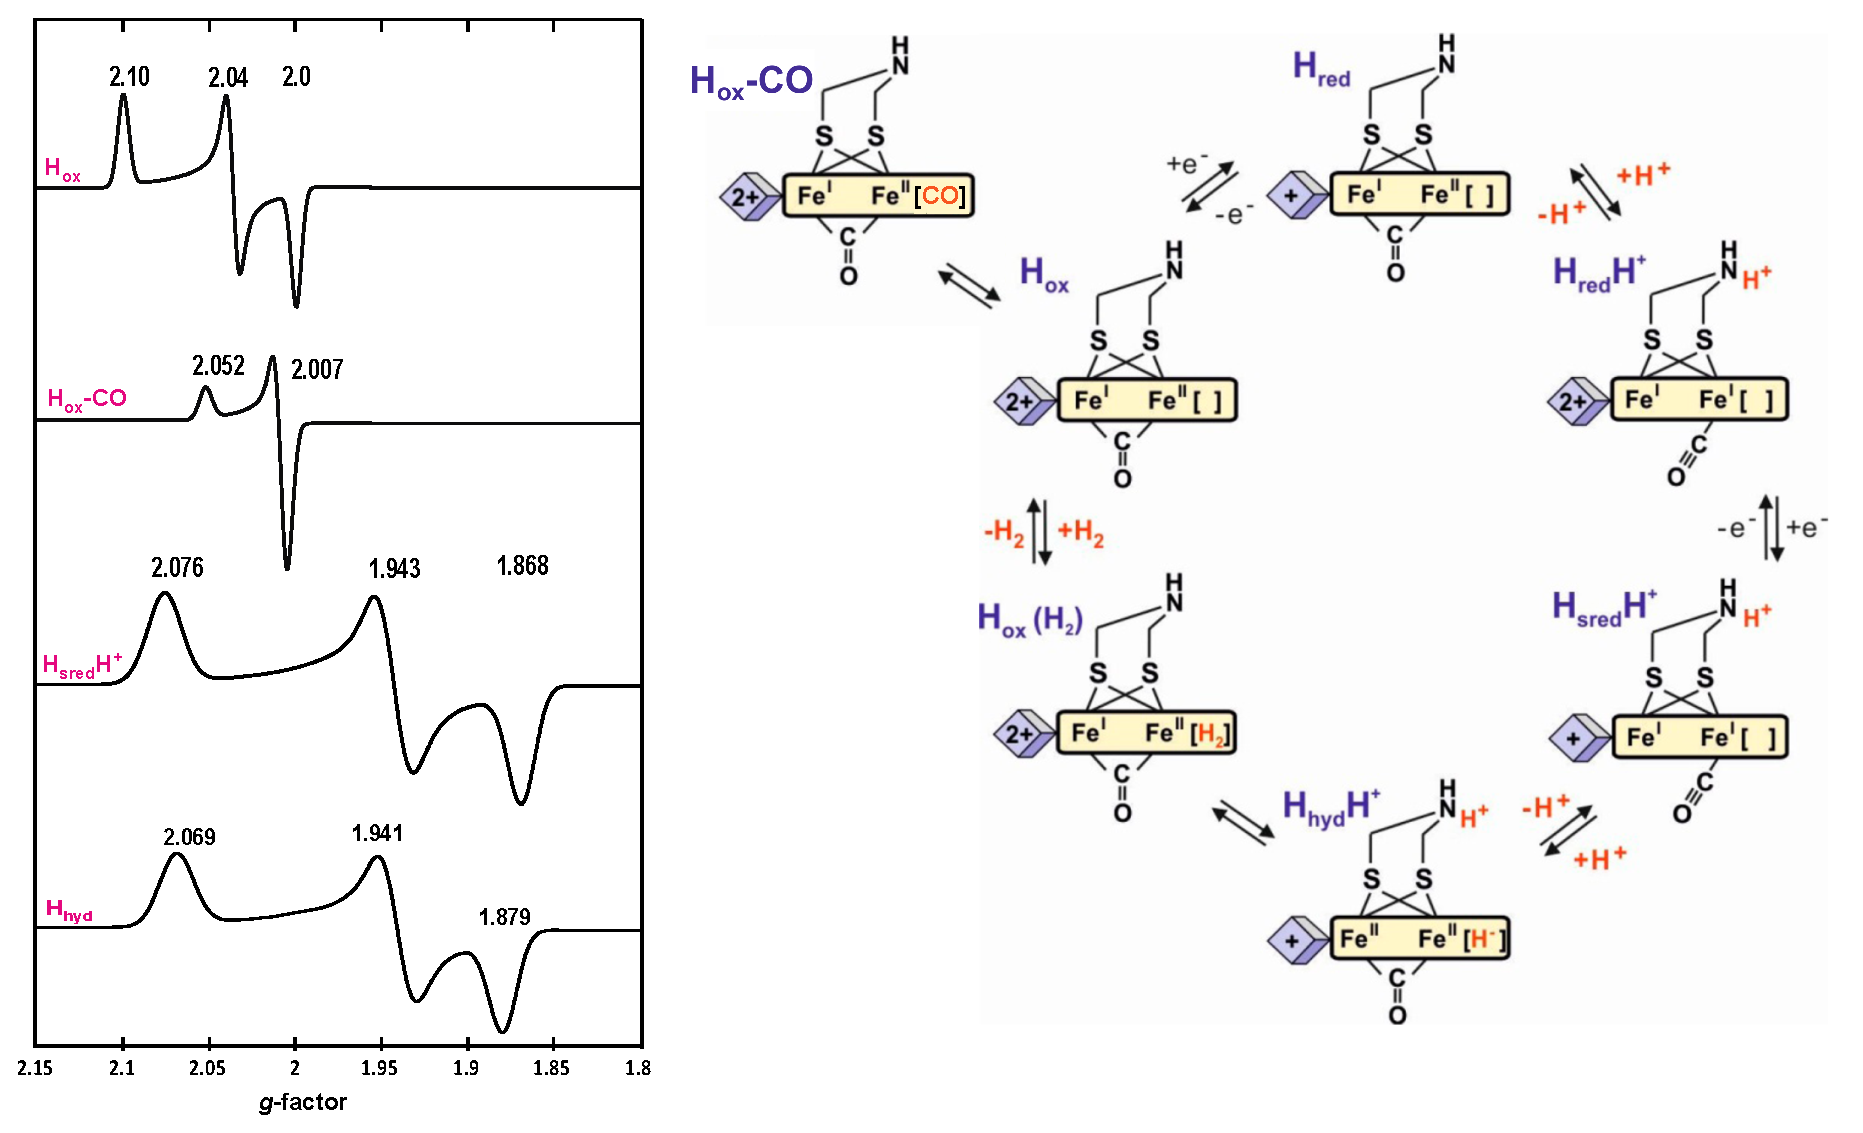
\includegraphics[width=\textwidth]{Kapitel/end-images/Ch6-EPRCat.eps}
 \caption[EPR Signals along the catalytic cycle of FeFe-Hydrogenase.]{Simulations of the EPR signal from stable paramagnetic intermediates of frozen solution samples along the catalytic cycle of [FeFe]-hydrogenase is displayed on the left. A simplified catalytic cycle showing the redox states of the distal and proximal iron and [4Fe-4S] clusters is displayed on the right.} 
 \label{fig:FeFeCatCycle}
\end{figure*}

Using frozen solution samples, EPR spectroscopy has been used to study the paramagnetic states of [FeFe]-hydrogenase from several organisms. \cite{lubitzhyd,Silakov57Fe,Adamska2015pdt,Adamska2015} These experiments have determined the magnetic principal \textit{g}-values, hyperfine, and quadrupole parameters for the catalytic states with EPR active co-factors and [4Fe-4S] clusters. Such important intermediate states include H$_{ox}$ and H$_{sred}$ in the catalytic cycle, a reversible carbon monoxide (CO) inhibited H$_{ox}$-CO state, and any state with reduced [4Fe-4S] clusters, including the \textit{apo}-HydA protein which lacks the H-cluster. Simulations of the frozen solution spectra of these states are shown in Fig.~\ref{fig:FeFeCatCycle}. In this work, focus was on H$_{ox}$ which is the primary catalytic state of the [FeFe]-hydrogenase where crystals of suitable size (0.8-3~nl) are available from CpI.

\paragraph{Summary of Magnetic Properties of the H$_{ox}$ Intermediate.} It was found that an \textit{Escherichia coli} (\textit{E. coli}) expressed \textit{apo}-HydA could be combined with an artificially synthesized H-cluster to form fully functional [FeFe]\-/hydrogenase. \cite{EsselbornArtificial,BirrellArtificial} This discovery has not only increased the yields of [FeFe]-hydrogenase synthesis but has allowed synthetically modified co-factors to be inserted into the \textit{apo} protein. These experiments allowed for a wealth of information to be obtained, including the identification of the head group in the bridging ADT-ligand which eluded X-ray crystallography diffraction measurements. \cite{AdamskaBridgingAmine} Additionally, it became possible to enrich the H-cluster with magnetic isotopes and study the corresponding magnetic interactions. These experiments allowed the synthesis of $^{57}$Fe in the binuclear co-factor, $^{13}$C, $^{14}$N, and $^{15}$N in the CN$^-$ and ADT ligands, and $^{13}$C in the CO ligands. A summary of the magnetic properties of the H$_{ox}$ stable catalytic intermediate can be found in Table~\ref{table:eprthing}. 
\begin{table}[htbp]
\caption[EPR parameters determined for FeFe-hydrogenase in Hox state.]{EPR parameters determined by frozen solution of [FeFe]-hydrogenase in the H$_{ox}$ stable catalytic intermediate through a series of pulse EPR experiments.}
\centering
\begin{tabular}{l|c|c||c}
 & Fe$_p$ $^\dagger$ & Fe$_d$ $^\dagger$ & {[}4Fe4S{]} \\ \hline \hline
oxidation state & II & I & 2+ \\
Spin state & $S=0$ & $S=1/2$ & $S_{eff}=0$ \\
$g$-values & -- & {[}2.100, 2.040, 1.999{]} & -- \\
A (MHz) & {[}12.3, 11.4, 12.6{]} & {[}12.3, 11.4, 12.6{]} & $\pm${[}11.2, 10.4, 11.6{]} \\
{[}$\alpha$, $\beta$, $\gamma${]} (deg) & {[}0, 0, 0{]} $\pm$30 & {[}0, 0, 0{]} $\pm$30 & {[}0, 0, 0{]} $\pm$30
\end{tabular}
\begin{flushleft}\footnotesize{$^\dagger$ From DFT calculations of Ref.~[6.\kern-0.4em\citenum{GrecoDFT}], it is assumed that the majority of the spin is located on Fe$_d$; however, significant $^{57}$Fe hyperfine interactions on both irons are measured by Silakov \textit{et al.} in Ref.~[6.\kern-0.4em\citenum{Silakov57Fe}].} \end{flushleft}

\begin{tabular}{l|c|c|c}
& C$^{15}$N$_d$ $^\ddagger$ & C$^{14}$N$_d$ $^\ddagger$ & ADT-Ligand ($^{14}$N)$^{\S}$\\ \hline \hline
A (MHz) &  {[}-1.3, -1.1, 6.2{]} & {[}-0.9, -0.8, 4.4{]} & {[}1.35, 1.15, 1.15{]}\\
{[}$\alpha$, $\beta$, $\gamma${]} (deg) & {[}-90, -50, 0{]}$^\ast$ & {[}-90, -50, 0{]}$^\ast$ & {[}0, 0, 0{]}\\
$P_{||}$ {[}MHz{]} &  -- & 0.9 & 1.23\\ 
$\eta$ & -- & 0.34 & 0.13 \\
{[}$\alpha$, $\beta$, $\gamma${]} (deg) & -- & {[}-46, -119, 0{]}$^\ast$ & {[}0, -90, 0{]}$^\ast$
\end{tabular}
\begin{flushleft}\footnotesize{$^\ddagger$ Data is obtained from Adamska \textit{et al.} of Ref.~[6.\kern-0.4em\citenum{Adamska2015}]. Other groups, such as Britt and colleagues in Ref.~[6.\kern-0.4em\citenum{BrittLigands2014}] have obtained similar values; however, Adamska \textit{et al.} use the same molecular frame described in this work. 

$^{\S}$ Data is obtained from Adamska \textit{et al.} of Ref.~[6.\kern-0.4em\citenum{Adamska2015pdt}]. }\end{flushleft}

\begin{tabular}{l|c|c|c|c}
 & $^{13}$CN$_p$ $^\ddagger$ & $^{13}$CN$_d$ $^\ddagger$ & ADT: $^{13}$C$_1$ $^\natural$ & ADT: $^{13}$C$_2$ $^\natural$ \\ \hline \hline
A (MHz) & {[}5.5, 5.5, 4.6{]} & {[}30, 28.5, 22.7{]} & {[}1.0, 1.3, 3.3{]} & {[}-1.49, -1.75, -0.45{]} \\
{[}$\alpha$, $\beta$, $\gamma${]} (deg) & {[}0, 0, 0{]} & {[}-46, -119, 0{]}$^\ast$ & -- & -- \\
\end{tabular}
\newline
\vspace*{0.5em}
\newline
\begin{tabular}{l|c|c|c}
 & $^{13}$CO$_p$$^{\ast\ast}$ & $^{13}$CO$_d$$^{\ast\ast}$ & $\mu^{13}$CO$^{\ast\ast}$ \\ \hline \hline
A (MHz) & {[}5.52, 5.52, 4.55{]} &  {[}20.5, 29.9, 26.0{]} & {[}9.0, 3.8, 4.5{]}\\
{[}$\alpha$, $\beta$, $\gamma${]} (deg) &  {[}25, 25, 0{]} & {[}37, 26, 0{]} & {[}0, 20, 0{]} \\
\end{tabular}\label{table:eprthing}

\begin{flushleft}\footnotesize{
$^\ast$ The Euler angles are in the new EasySpin Euler definition (since version 5.0), which required the transformation $[\alpha,\beta,\gamma]= -[\gamma,\beta,\alpha]$ from the published results.

$^{\ast\ast}$ Data is obtained from Britt \textit{et al.} of Ref.~[6.\kern-0.4em\citenum{BrittC13}].

$^\natural$ The principal values were found using Q-band ENDOR spectroscopy and the sign was determined by the MIMS-TRIPLE experiment in Ref.~[6.\kern-0.4em\citenum{Reijerse13C2019}].
} \end{flushleft}
\end{table}

The data in Table~\ref{table:eprthing} represents the current knowledge on the magnetic properties of the [FeFe]-hydrogenase in the H$_{ox}$ stable catalytic intermediate. However, this table is not exhaustive and further information on both the magnitude and orientation of the \textit{g}-, hyperfine-, and quadrupole-tensors is still needed. To date, quantum chemical calculations have difficulties in predicting the principal values of the \textit{g}-tensor and are only used to qualitatively assign spin densities when simulating interactions with surrounding nuclei.\cite{GrecoDFT,FiedlerDFT}  From the current literature, it is not clear which amino acids are involved in the first ligand-sphere and, therefore, single-crystal EPR experiments are needed to properly determine the full-magnetic interactions of the H-cluster. 

In Chapter~5, advancement to the state-of-the-art EPR instrumentation was achieved with the self-resonant micro-helix. From this development the ability to measure protein single crystals with dimensions less than 0.3~mm$^3$ is now feasible. In this chapter, the demonstration of (i) a full angular $g$-tensor determination is performed and, due to the six-fold signal enhancement of the micro-helix, that (ii) advanced pulse EPR experiments, like ESEEM and HYSCORE, are attainable on the same crystal. Herein, for the first time, the $g$-tensor values from field-stepped ESE rotational data and $^{14}$N HYSCORE data for a [FeFe]-hydrogenase in the active oxidized state (H$_{ox}$) from \textit{Clostridium pasteurianum} in a 0.3 $\times$ 0.1 $\times$ 0.1~mm$^3$ crystal volume are exhibited.\footnote{Only one other study is known where both measurements of the $g$-tensor and ESEEM/HYSCORE experiments were performed on the same crystal. The [NiFe]-hydrogenase protein single-crystals used in this study had a volume of 8~$\mu$l. Experiments were performed at both at X- and W-band. These studies can be found in Ref.~[6.\kern-0.4em\citenum{Brecht2001}].} These data demonstrate the utility of the micro-helix in studying protein single-crystals at sizes relevant for X-ray crystallography. 

\section{Methods}
The [FeFe]-hydrogenase from \textit{Clostridium pasteurianum} (CpI) was crystallized with a maximum  size of 0.3 $\times$ 0.1 $\times$ 0.1~mm$^3$ by the method of Esselborn \textit{et al.}\cite{FeFeCry} under auto-oxidative conditions, i.e. without reducing agents. This leaves the enzyme in the characteristic active oxidized state (H$_{ox}$), giving rise to a $S=1/2$ ground state of the H-cluster. The accessory iron-sulfur clusters in the protein are oxidized and, due to anti-ferromagnetic coupling, remain EPR silent with an effective spin of zero. \cite{lubitzhyd}  Under a microscope in an anaerobic chamber, the protein crystal is drawn by capillary action into a 0.3~mm inner diameter capillary with mother liquor and cryoprotectant, centered in the micro-helix, and flash frozen. The micro-helix assembly is affixed to the EPR probehead, placed in a pre-cooled cryostat, and attached to the EPR bridge. 

\begin{figure}[htbp]
\centering
 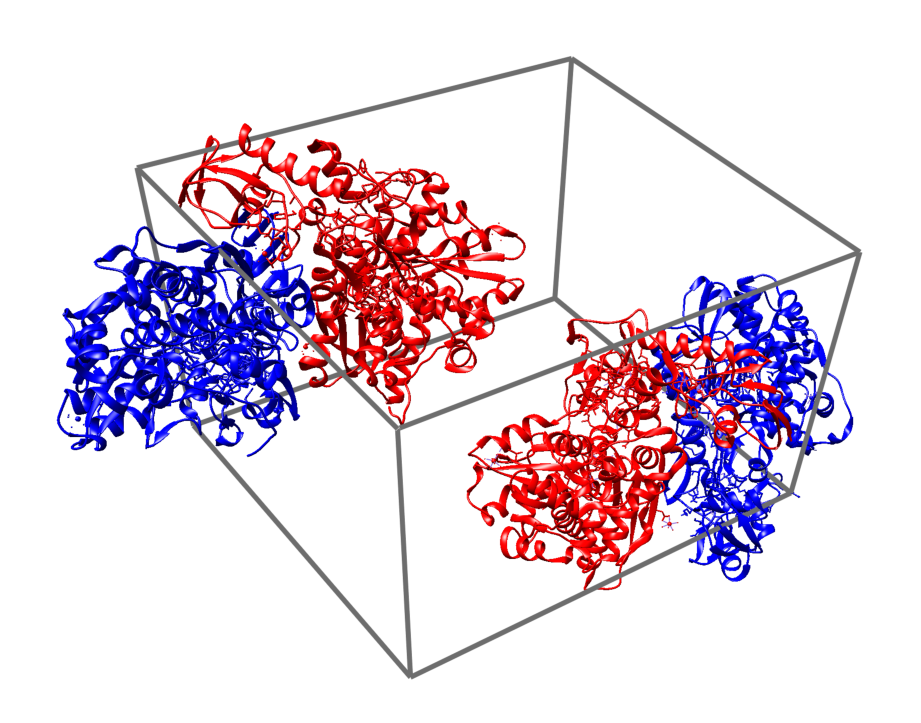
\includegraphics[width=0.5\textwidth]{Kapitel/Ch6-Images/Ch6-UnitCell.eps}
 \caption[Unit Cell from PDB 4XDC.]{Shown is the unit cell of PDB ID 4XDC with the molecules in an asymmetric unit (red and blue) and copied by the P$1\,2_1\,1$ symmetry.} 
 \label{fig:xTalFeFeUnit}
\end{figure}

The [FeFe]-hydrogenase of \textit{Clostridium pasteurianum} (CpI) has a molecular weight of 64~kDa. The unit cell has P$1\,2_1\,1$ symmetry with two molecules in the asymmetric unit (PDB ID: 4XDC), shown in Fig.~\ref{fig:xTalFeFeUnit}. Each of the four enzymes per unit cell contains one H-cluster, Fig.~\ref{fig:CpIGeo}B, which results in four distinct signals. The single crystal had, based on the unit cell dimensions, approximately 17$\times10^{12}$ enzymes within the crystal. The signals correspond to 4.25$\times10^{12}$ spins per peak. 

\begin{wrapfigure}{O}[0pt]{3.5cm}
\centering

\includegraphics[width=3.5cm]{Kapitel/Appendix/eFitRoutinesQR.eps}
\end{wrapfigure}

In the current setup, the entire probehead is rotated within the magnet with the static magnetic field in the laboratory frame $L_1$-direction and rotation takes place on axis of the microwave magnetic field in the $L_3$-direction, illustrated in Fig.~\ref{fig:CrystalOrientation}. The probehead setup is axially symmetric and the whole micro-helix probehead is rotated in 5$^{\circ}$ steps over 180$^{\circ}$ in one-plane within the magnet as shown in Fig.~\ref{fig:RotateMe}A.

For the fitting, the laboratory frame is set in the EasySpin simulations and the collected spectra are fitted using the Matlab programs supplied in Appendix~D.\footnote{The Matlab program files can be found at: \textit{https://github.com/jsidabras/esFit-routines}.} The \textit{esfit} routine was modified with a sub-routine employing partial parallelization of the simulations. This allowed for 12 spectra in 3 chunks to be simulated simultaneously for a total of 36 spectra per fit. A particle swarm optimization algorithm with 10,000 particles (fits) was used to find the solution. Each run was allowed to converge in 10 iterations and was checked if a local minimum was found. The EasySpin solution took about 1~second for each fit for a total of approximately 2.5~hours per iteration. Simulations were re-run until a good fit was established.

The EasySpin fitting simulation is set up with 9 unknowns: the three axes of the crystal frame that relates how the crystal is orientated in the laboratory frame, the three axes of the $g$-tensor of the first molecule ($g$-tensor A) and how it relates to the Molecular-Frame A, and the three axes of the $g$-tensor of the second molecule ($g$-tensor B) and how it relates to the Molecular-Frame B. 

\begin{figure}[ht]
 \centering
 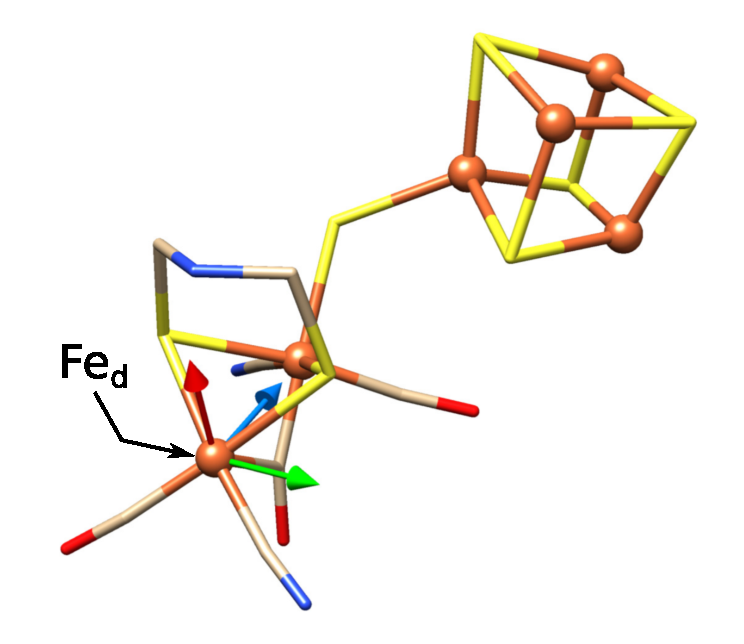
\includegraphics[width=0.5\textwidth]{Kapitel/Ch1-images/Ch2-MolFrame.eps}
 \caption[Molecular Frame of FeFe-hydrogenase H$_{ox}$ state.]{Molecular Frame of FeFe-hydrogenase H$_{ox}$ state from PDB ID: 4XDC. With the axes labeled as $g_x$: red, $g_y$: green, and $g_z$: blue. The distal iron (Fe$_d$) is indicated and the $g$-components are $g_z>g_y>g_x$.}
 \label{fig:MolecularFrame}
\end{figure}

From the crystal structure, the molecular frame of the H-cluster can be determined. The molecular frame is calculated using the distal iron (Fe$_d$) as the origin and is plotted in Fig.~\ref{fig:MolecularFrame}. The three axes for the molecular frame were chosen as (i) an axis from the distal iron (Fe$_d$) to the proximal iron (Fe$_p$), (ii) the normal of a plane calculated from the proximal iron, distal iron, and the nitrogen of the ADT-ligand  (Fe$_p$-Fe$_d$-N$_1$), and (iii) the cross product of (i) into (ii). The $g_z$-component was chosen to be the axis from Fe$_d$ to Fe$_p$ and the $g$-components are ordered by $g_z>g_y>g_x$. 

The first molecular-frame (Molecular-Frame A) is shown as a red protein in Fig.~\ref{fig:xTalFeFeUnit}. The second molecular-frame (Molecular-Frame B) is needed since the [FeFe]-hydrogenase is crystallized with an asymmetric unit, shown as a blue protein in Fig.~\ref{fig:xTalFeFeUnit}. The molecular frame is defined by the same procedure as the Molecular-Frame A, but at the origin of the distal iron in the H-cluster of protein B.

Based on similar research at W-band with photosystem II, it can be assumed that the $g$-tensor of the second molecule will be almost the same as the first molecule. \cite{Hofbauer6623,B908093G} The deviation of the $g$-tensor of the second molecule ($g$-tensor B) with respect to the first ($g$-tensor A) is limited to 15 degrees. While the crystal frame and $g$-tensor A were set to vary a whole rotation. The principal $g$-values were obtained from previous frozen solution EPR experiments from Ref.~[6.\kern-0.4em\citenum{lubitzhyd}] ($g$-values: [1.999, 2.039, 2.097] corresponding to $x$, $y$, and $z$, respectively).

For the HYSCORE experiment the magnetic field is set to one of the peaks measured in the two-pulse ESE experiment, $\tau$ is 280~ns, $t_1$ and $t_2$ start at 300~ns with 256 48~ns steps, and $\pi$-pulse is 80~ns at a microwave power of 7~mW. 

\clearpage
\section{Results and Discussion}
\subsection{Pulse EPR in Single Crystals of [FeFe]-Hydrogenase.}
\begin{figure}[htbp]
\centering
 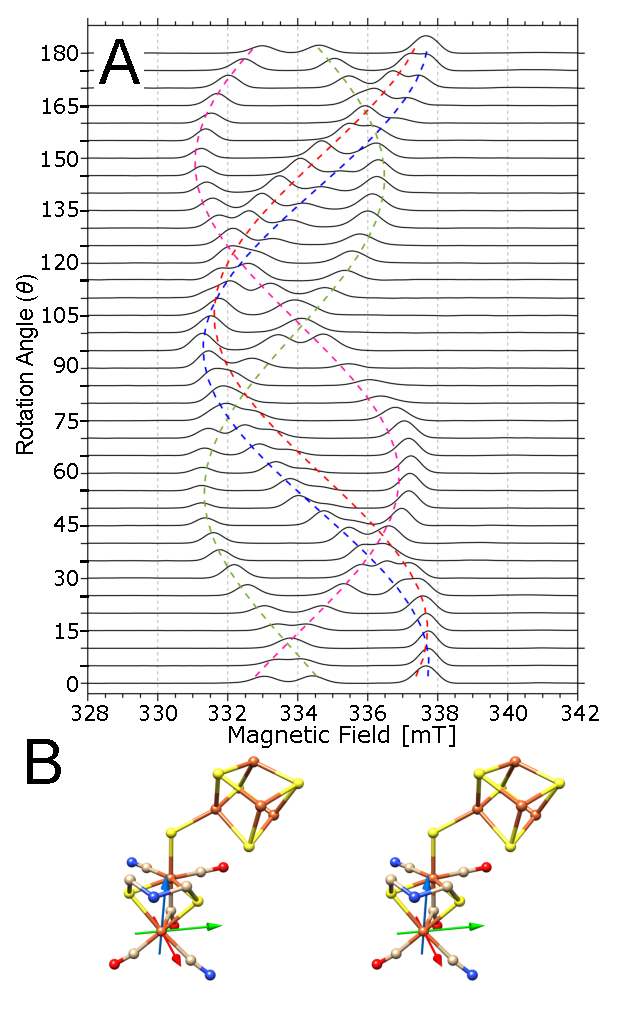
\includegraphics{Kapitel/Ch5-Images/04-FeFe-xTal-DataBig.eps}
 \caption[Pulse EPR on single-crystal of the H-cluster in FeFe-hydrogenase.]{A) Pulse EPR on single-crystal [FeFe]-hydrogenase of \textit{Clostridium pasteurianum} (CpI) in the H$_{ox}$ stable catalytic intermediate showing collected data in one plane for a full rotation of 180$^{\circ}$ in 5$^{\circ}$ steps at a temperature of 15~K. B) A stereo view of the analyzed $g$-tensor (g$_x$: green, g$_y$: blue, g$_z$: red) is mapped on the crystal structure (PDB ID: 4XDC). The order of the principal values of the $g$-tensor is $g_z\geq g_y\geq g_x$.} 
 \label{fig:xTalFeFe}
\end{figure}

\begin{wrapfigure}{I}[0pt]{3.5cm}
\centering
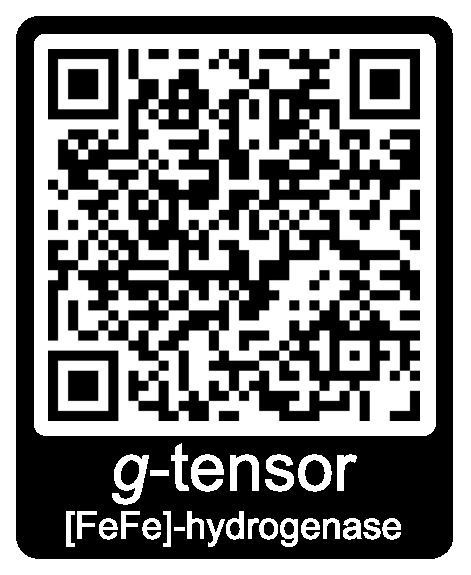
\includegraphics[width=3.5cm]{Kapitel/Appendix/FeFegtensorQR.eps}
\end{wrapfigure}

First, a field-swept two-pulse electron spin-echo EPR experiment was performed every 5$^{\circ}$ on a protein single-crystal of the [FeFe]-hydrogenase of \textit{Clostridium pasteurianum} (CpI) in the oxidized H$_{ox}$ stable catalytic intermediate and plotted in Fig.~\ref{fig:xTalFeFe}A. A very good signal-to-noise ratio of approximately 290 is calculated for a collection time of only 8~minutes for each spectrum at a temperature of 15~K. 

From these spectra, the data can be fitted to simulations that relate the different frames of reference to each other as defined in the EasySpin simulation package. Rotational matrices for the relationship of these frames are tabulated in Table~\ref{table:frames}. The rotational matrices are calculated from the Euler angles found from the fitting of the laboratory and $g$-tensor frames. The peak positions of the EasySpin simulated data are plotted as an angle-dependent ``resonance roadmap'' which overlays on top of the field-swept two-pulse electron spin-echo EPR experiment, shown in Fig.~\ref{fig:xTalFeFe}A. Each of the four dashed lines represent the EPR signals originating from the unit cell.

\begin{table}[htbp]
\caption[Rotational matrices for the crystal frame.]{Rotational matrices  for the crystal frame with respect to the laboratory frame and the $g$-tensor with respect to the molecular frame. The crystal frame and $g$-tensor are found by fitting the data in Fig.~\ref{fig:xTalFeFe}A with the molecular frame from PDB ID 4XDC.}
\centering
\hspace{-12.825em}
\begin{tabular}{r|ccc}
 & \multicolumn{3}{c}{Crystal Frame} \\
\multicolumn{1}{l|}{} & $a$ & $b$ & $c$ \\ \hline \hline
L$_1$ & $+$0.273 & $-$0.162 & $-$0.948 \\
L$_2$ & $-$0.022 & $-$0.987 & $+$0.162 \\
L$_3$ & $-$0.962 & $+$0.023 & $-$0.273
\end{tabular}\label{table:frames} \\
\vspace{0.5cm}
\begin{tabular}{r|ccc|ccc}
 & \multicolumn{3}{c|}{Molecular-Frame A} & \multicolumn{3}{c}{Molecular-Frame B} \\
 & $x$ & $y$ & $z$ & $x$ & $y$ & $z$ \\ \hline \hline
$a$ & $-$0.331 & $-$0.938 & +0.107 & $-$0.595 & $-$0.666 & $-$0.450 \\
$b$ & $-$0.770 & +0.203 & $-$0.605 & +0.456 & $-$0.740 & +0.494 \\
$c$ & +0.545 & $-$0.283 & $-$0.789 & $-$0.662 & +0.089 & +0.744
\end{tabular}\\
\vspace{0.5cm}
\begin{tabular}{r|ccc|ccc}
 & \multicolumn{3}{c|}{$g$-Tensor A} & \multicolumn{3}{c}{$g$-Tensor B} \\
 & $x$ & $y$ & $z$ & $x$ & $y$ & $z$ \\ \hline \hline
$a$ & $+$0.476 & $-$0.484 & $+$0.735 & $+$0.377 & $-$0.605 & $-$0.701 \\
$b$ & $-$0.400 & $+$0.625 & $+$0.671 & $-$0.388 & $+$0.584 & $-$0.713 \\
$c$ & $+$0.783 & $+$0.613 & $-$0.103 & $+$0.841 & $+$0.541 & $-$0.015
\end{tabular}
\end{table}

The proposed $g$-tensor orientation is plotted as a stereo view in Fig.~\ref{fig:xTalFeFe}B.\footnote{For a 3D view of the proposed $g$-tensor see: https://act-epr.org/FeFeHydrogenase.html} The $g$-tensor (g$_x$: green, g$_y$: blue, g$_z$: red) is presented with the origin at the distal iron (Fe$_d$), where DFT calculations predict the majority of the spin density in the H$_{ox}$ stable catalytic intermediate exist. \cite{FiedlerDFT,GrecoDFT} 

\paragraph{Comparison to Previous Literature.} With $^{14}$N and $^{15}$N HYSCORE measurements of the CN$_d^-$ and ADT-ligand in frozen solution, Adamska \textit{et al.} could simulate and calculate a hypothetical $g$-tensor that would give rise to the measured spectra. \cite{Adamska2015} By proposing that the g$_z$-axis lies along the Fe$_p$-Fe$_d$ axis, an angle of 117$^\circ$ is made by CN$_d^-$-Fe$_d$-g$_z$, shown in Fig.~\ref{fig:gTensor}A. This angle produced simulated HYSCORE data that matched well to the measured data. Additionally, The g$_x$-axis was chosen to point along the Fe$_d$ to ADT-amine nitrogen axis bisecting the nitrogen which is believed to be part of the formation of the hydride.

\begin{figure}[ht]
\centering
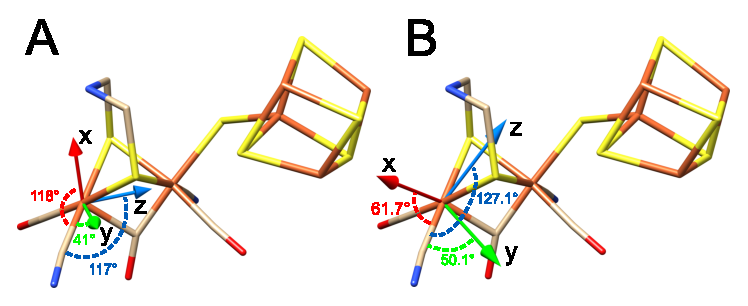
\includegraphics{Kapitel/Appendix/Images/S6-gTensorCompare.eps}
\caption[Comparison of the proposed $g$-tensor.]{A) The proposed $g$-tensor by Adamska \textit{et al.} overlaid onto the H-cluster from PCB ID 3C8Y. (Adapted from Ref.~[6.\kern-0.4em\citenum{Adamska2015}] with permission from the PCCP Owner Societies.) B) The proposed $g$-tensor of this work overlaid onto the H-cluster from PCB ID 4XDC.\cite{FeFeCry}}
\label{fig:gTensor}
\end{figure}

The data collected using single-crystal EPR in this work is in good agreement with the HYSCORE data representing the g$_z$-axis collected by Adamska \textit{et al.}. Only a deviation of 10.1$^{\circ}$ is measured from the axes previously proposed, shown in Fig.~\ref{fig:gTensor}B. However, the newly proposed $g$-tensor orientation has the $x$-axis pointing outward at the open coordination site and a 9.1$^{\circ}$ deviation from bisecting the H-cluster. The $g$-tensor measured by single-crystal experiments shows that the g$_z$-axis lies on the plane created by the CO$_d$, CN$_d^-$, and bridging sulfur. 

The deviation from the frozen solution data is because it was under-determined. With single-crystal data, no assumptions are made in the fitting of the $g$-tensor. Further analysis and refinement is possible with the collection of hyperfine and quadrupole data originating from the same crystal and relating the whole dataset to quantum chemical calculations.

\subsection{Advanced Pulse EPR in Single Crystals.}
Single-crystal ESEEM and HYSCORE experiments were performed due to the excellent signal-to-noise of the field-stepped ESE. HYSCORE was performed every 30$^{\circ}$ on each of the peaks shown in the field-swept ESE EPR dataset. Each spectrum was collected over approximately one hour, using a standard four-pulse HYSCORE sequence. \cite{schweiger2001principles} To obtain information on the hyperfine- and quadrupole-tensors, HYSCORE or ESEEM data must be collected on at least one peak and followed through a 180$^{\circ}$ rotation. Multiple peaks can be used to over-determine the system. A series of HYSCORE experiments following the fuchsia-colored resonance roadmap of Fig.~\ref{fig:xTalFeFe}A is shown in Fig.~\ref{fig:FeFeHYSCOREFollow}. 

\begin{figure}[ht]
\centering
 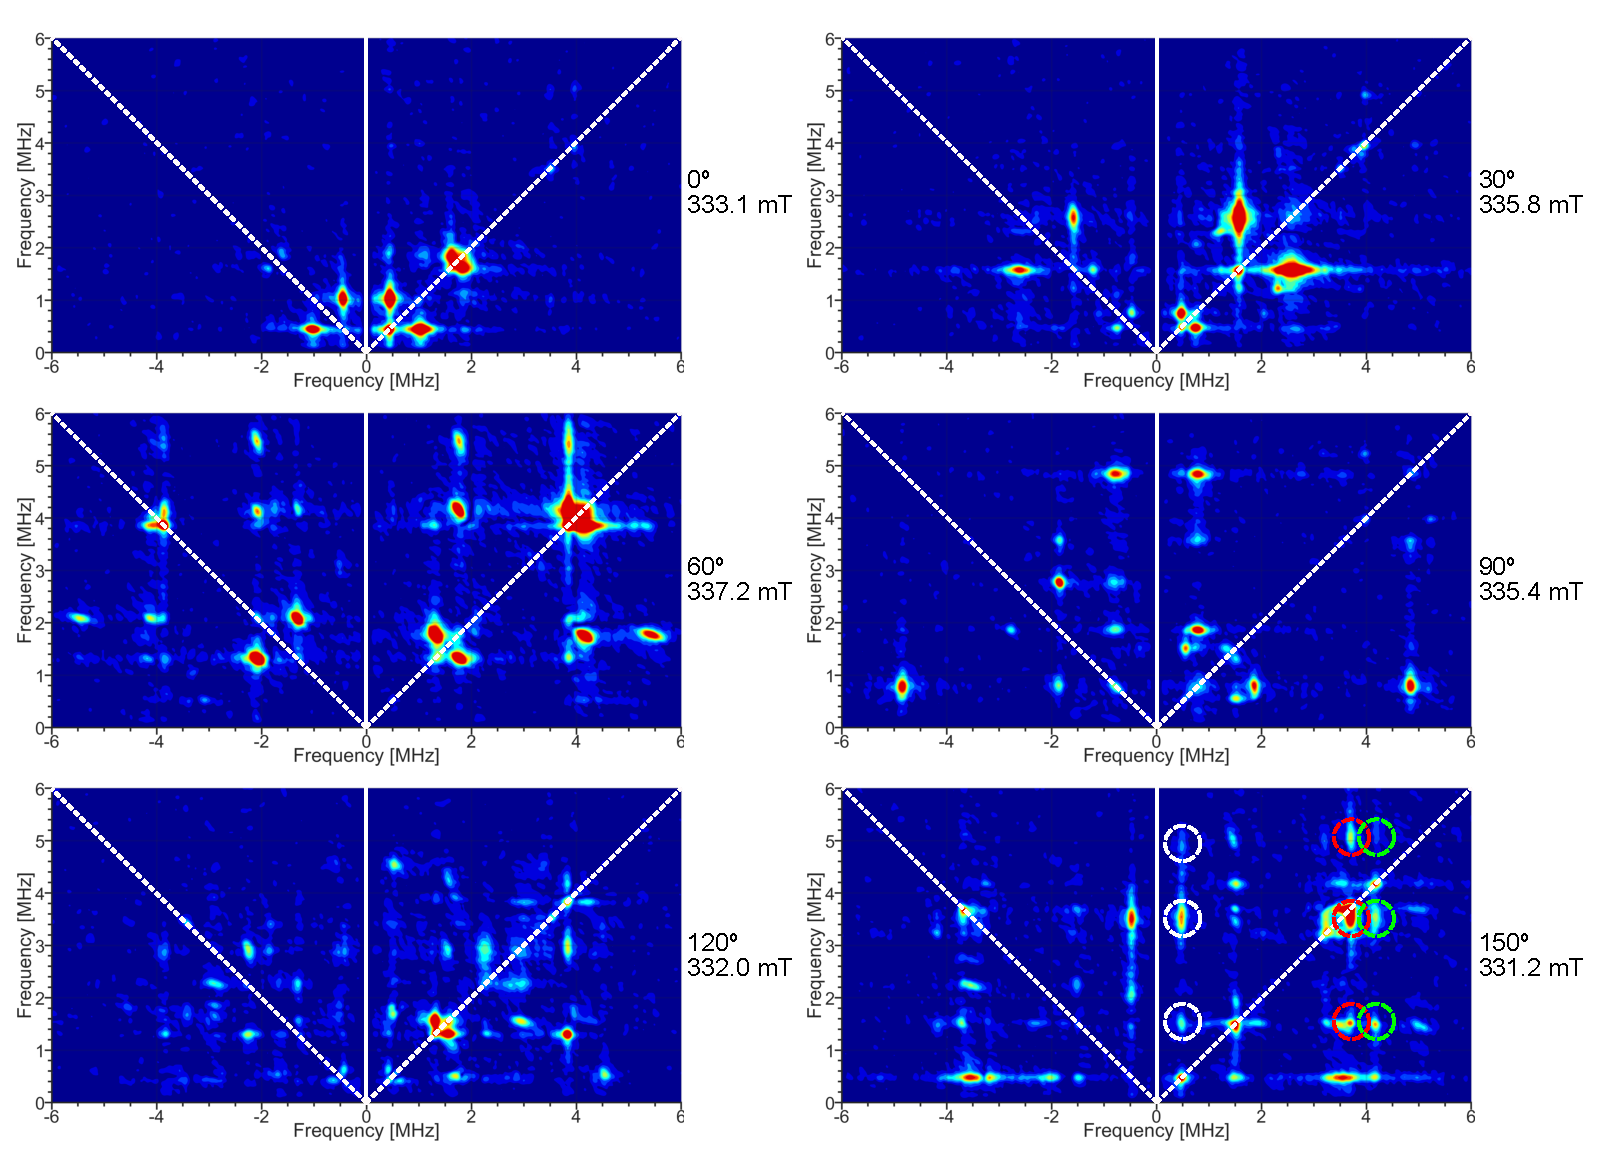
\includegraphics[width=\textwidth]{Kapitel/Ch5-Images/FeFe-FollowHyscore.eps}
 \caption[Single-crystal HYSCORE EPR following a single peak.]{Single-crystal HYSCORE EPR following the fuchsia-colored resonance roadmap of Fig.~\ref{fig:xTalFeFe}A.} \label{fig:FeFeHYSCOREFollow}
\end{figure}

In an HYSCORE experiment, the 2D density representation shows correlations between the nuclear-spin transitions (m$_\text{I}$) in both projections of the electron spin. Both, the $^{14}$N nucleus ($I=1$) from a distal cyanide-ligand (CN$_\text{d}^-$) and the secondary amine group in the ADT-ligand can potentially contribute to the HYSCORE spectrum generating three transitions per ligand for each electron-spin transition (m$_\text{S}$) manifold. According to an earlier study on H$_{ox}$ in frozen solution, the features of the distal cyanide-ligand spread out up to 6 MHz, while the transitions of the ADT-amine nitrogen are found between 2 and 4~MHz. \cite{Adamska2015,Adamska2015pdt}

Currently, the full hyperfine- and quadrupole-tensor has not been solved. However, a comparison of the data that was collected with previous work can be used to gain further insight. For example, in Fig.~\ref{fig:FeFeHYSCOREFollow} at 0 and 30 degrees a strong signal can be seen in the weak coupling (++) quadrant under a coupling frequency of 4~MHz. These signals are attributed to the ADT-ligand and fit the principal values described in Adamska \textit{ et al.} \cite{Adamska2015pdt} As the HYSCORE data is rotated these signals are reduced and signals with larger couplings are found in the 4 to 6~MHz range, including signals in the strong coupling ($-+$) quadrant. These signals are best represented by the distal cyanide-ligand (CN$_\text{d}^-$) as described in a second paper by Adamska\textit{ et al.} \cite{Adamska2015}. 

\section{Conclusions and Outlook}
In this work, it has been demonstrated that a full angular $g$-tensor determination can be performed on crystals with volumes smaller than 30~nl with excellent signal-to-noise ratio at X-band frequencies. The proposed $g$-tensor is a refinement on previous work by Adamska \textit{et al.}, which used orientation-selection HYSCORE on frozen-solution samples at X-band and Q-band to back project the $g$-tensor. In the present work, no assumptions were made and the $g$-tensor was measured directly. Although only a single plane was covered, the P$1\,2_1\,1$ symmetry of the crystal and the orientation of the crystal in the Laboratory Frame has allowed for a good fit. 

This work also demonstrates the ability to perform HYSCORE experiments on the same crystal and highlights the feasibility of such advanced pulse EPR measurements. Future ESEEM and HYSCORE experiments will address the $^{14}$N couplings of the CN$^-$ and ADT-ligand in greater detail. Possibly this will involve selective $^{15}$N labeling as has been demonstrated before. \cite{Adamska2015,AdamskaBridgingAmine} From such experiments it is possible to extract the magnitude and orientation of the nitrogen hyperfine- and quadrupole-tensors in the molecular axis frame and relate them to the electronic structure as predicted through quantum chemical calculations. Such studies will further protein engineering and artificial enzyme research for creating bio-inspired and bio-mimicking hydrogenase systems. \cite{C7SE00582B}

This work shows the application of the synergy between X-ray crystallography diffraction data and EPR. The self-resonant micro-helix further strengthens this synergy by reducing the crystal dimensions to less than 0.3~mm and reducing the crystallograpy barrier to studying important enzymes with stable paramagnetic states.


{\renewcommand{\bibsection}{\clearpage\section*{\bibname}\markboth{\bibname}{\bibname}}
\renewcommand{\bibname}{CHAPTER 6. REFERENCES}
\bibliographystyle{elsarticle-num}
\bibliography{Kapitel/Ch5-References}
}
